\subsection{Architettura}
L'architettura di Apache Spark si ispira fortemente a quella di Hadoop. Difatti, presenta una struttura gerarchica \textbf{Master-Slaves} dove il nodo master che gestisce i nodi in esecuzione e controlla l’amministratore del cluster. 

All'interno del nodo master viene istanziato un \textit{driver}, processo che si occupa di distribuire il codice dell’utente tra i nodi e convertirlo in più attività (\textit{jobs}). Il driver distribuisce questi compiti sui nodi slave (worker) e organizza la loro esecuzione.  Le applicazioni Spark vengono eseguite come serie indipendenti di processi in ambiente distribuito, coordinate dallo \textbf{SparkContext}, un processo che funziona come una porta d'accesso a tutte le funzionalità di Spark.

I \textbf{nodi worker} eseguono le attività assegnate dal driver su questi nodi. Eseguti i jobs assegnati, restituiscono il risultato allo SparkContext. 
È però necessario implementare un gestore del cluster o \textbf{cluster manager} (Spark Standalone Cluster Manager, Hadoop Yarn, Apache Mesos, Kubernetes) per mediare tra i workers e driver. 
\begin{figure}[hbt!]
    \centering
    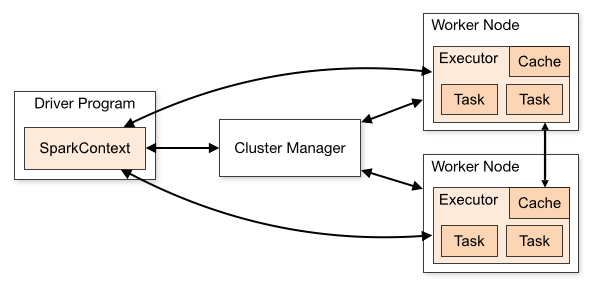
\includegraphics[width=1\textwidth]{img/sparkarchitecture.png}
    \caption{Architettura Spark}
    \label{fig:spark_architettura}
\end{figure}\\

% Spark può essere eseguito in due modalità:
% \begin{itemize}
%     \item \textbf{Cluster Mode}: il cliente che presenta l'applicazione Spark avvierà il driver e manterrà lo SparkContext. Quindi, fino a quando l'esecuzione del lavoro non sarà finita, la gestione dei jobs sarà svolta dal driver. Inoltre, il client deve rimanere sempre in contatto con il cluster: il client dovrà essere online fino a quando quel particolare processo non sarà completato.
%     \item \textbf{Client Mode}: il driver Spark o il master dell'applicazione Spark verrà avviato in una qualsiasi delle macchine worker. Quindi, il client che sta presentando l'applicazione può presentare l'applicazione e può o andare via dopo aver avviato l'applicazione o continuare con qualche altro lavoro. Questo meccanisco è anche chiamato \textit{Fire and Forget}.
% \end{itemize}